\xchapter{Revisão sistemática de literatura}
{ }%Revisão sistemática de literatura}

\section{Protocolo da revisão sistemática de literatura}

A revisão sistemática de literatura é um método de seleção de artigos a partir de um protocolo de busca que tem como objetivos resumir evidências empíricas, identificar lacunas existentes nas pesquisas realizadas até o momento e fornecer estruturas para realizar novas pesquisas. Uma revisão sistemática de literatura é composta por três fases: planejamento da revisão, condução da revisão e análise dos resultados~ \cite{Kitchenham:2007} .

Na fase do planejamento é escolhido qual tema será estudado. define-se a pergunta de pesquisa, que deverá ser respondida após a análise dos artigos estudados. Seleciona-se as palavras chave para a criação da string de busca que será utilizada nas bases de dados escolhidas pelo pesquisador e por fim devem ser escolhidos os critérios de inclusão e de exclusão.

Na fase de condução da revisão, as strings de busca criadas deverão ser aplicadas nas bases de dados escolhidas na fase anterior.
Após adquirir o material através da aplicação das strings de busca, os resultados retornados são classificados em dois grupos: os artigos que foram aceitos e os que foram rejeitados.

A classificação é realizada através da aplicação dos critérios de inclusão e de exclusão escolhidos na fase anterior.
Quanto à escolha dos critérios de inclusão e de exclusão que serão aplicados no artigo, cabe enfatizar que deve-se seguir a  seguinte regra: Se um artigo se encaixar em pelo menos um critério de exclusão, este deverá ser eliminado do grupo de artigos aceitos, mesmo que se encaixe em algum critério de inclusão, e para um artigo pertencer ao conjunto de artigos aceitos devem satisfazer a todos os critério de inclusão e a nenhum critério de exclusão~\cite{Kitchenham:2007}. 

Essa revisão sistemática de literatura tem como propósito: identificar as lacunas existentes no Problema de Roteamento e Escalonamento da Equipe de Atenção Domiciliar e desvendar novas oportunidades de pesquisa e auxiliar pesquisadores na construção de novas soluções para o problema. 

Além dos artigos coletados a partir da chave de busca, outros materiais também foram utilizados para complementar a pesquisa, tais como artigos encontrados a partir de outras bases de dados ou a partir de outras strings de busca, literatura cinza ou livros.

\section{Execução do Mapeamento Sistemático}

O objetivo desse mapeamento sistemático é buscar materiais para investigar a possibilidade propor uma solução heurística para o Problema de Escalonamento e Roteamento de Profissionais de Saúde, de forma que seja possível aumentar  o número de clientes atendidos e reduzir o tempo de transporte da equipe de profissionais de saúde. 
A partir do objetivo da pesquisa foi encontrado a seguinte questão de pesquisa:~\emph{É possível maximizar o número de visitas da equipe de atendimento domiciliar a partir da aplicação de soluções heurísticas?}

Para responder a questão de pesquisa foram examinados trabalhos sobre utilização de heurísticas e meta-heurísticas aplicadas ao escalonamento e roteamento  de equipes de enfermeiras e de atendimento domiciliar, tendo como grupo de controle heurísticas relacionadas com o problema.

O resultados esperados ao final da pesquisa é: A identificação de lacunas existentes no Problema de Escalonamento e Roteamento da Equipe de Atenção Domiciliar e facilitar o acesso das heurísticas já elaboradas por outros pesquisadores para que dessa maneira facilite a construção de novas soluções para o problema.

Para a elaboração da pesquisa foram utilizadas as seguintes palavras chave: \textit{``home health care''}, \textit{``home care'', ``nurse scheduling''} e \textit{``nurse routing''}, organizadas na seguinte string de busca: \textit{``(``home health care'' OR ``home care'') AND (``routing OR scheduling'')''} e \textit{``nurse AND (routing OR scheduling)''}. 

A Pesquisa foi restrita a artigos escritos na língua inglesa e portuguesa, selecionados a partir seguintes bases de pesquisa: \textit{Science Direct, Springer}, \textit{IEEE Xplore}, \textit{Scopus} e \textit{ACM Digital Library}. Além dos artigos selecionados a partir da strings de busca nas bases citadas, a pesquisa conta com outros materiais, tais como livros, materiais retirados da literatura cinza e artigos adquiridos de forma ad-oc.

A pesquisa realizada a partir da string de busca retornou 151 resultados distribuídos da seguinte forma: 73 artigos da \textit{Science Direct}, 50 artigos do \textit{IEEE Xplore}, 16 artigos da \textit{Springer}, 7 artigos da \textit{Scopus} e 5 artigos da \textit{ACM digital Library}.% como pode ser observado na Figura~\ref{base_de_dados_de_origem}.

%Colocar figura nos slides
% \begin{figure}[H]
% \begin{center}
% 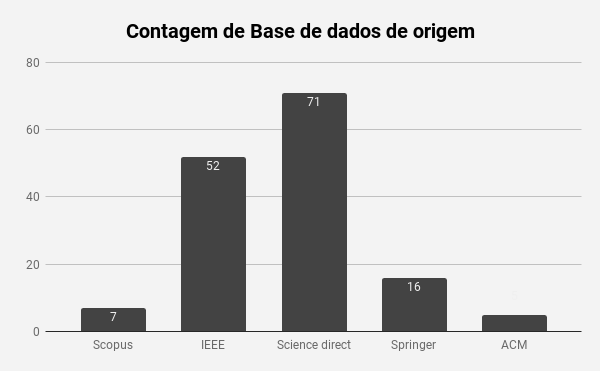
\includegraphics[width=0.6 \textwidth]{contagem_base_de_dados_de_origem.png}
% \caption{Contagem de artigos por bases de dados \label{base_de_dados_de_origem}}
% \end{center}
% \end{figure}

Após a realização da busca dos artigos nas bases de dados especificadas, os artigos encontrados foram selecionados segundo os seguintes critérios de inclusão e de exclusão.

\textbf{Critérios de inclusão:}
\begin{itemize}
\item Artigos que possuam foco em problemas de escalonamento de profissionais de saúde;
\item Artigos que possuam foco em problemas roteamento de veículos das equipes de profissionais de saúde;
\item Artigos publicados em revistas ou conferências.
\item Artigos da área de Pesquisa Operacional
\end{itemize}

\textbf{Critérios de exclusão:}
\begin{itemize}
\item Artigos que não estejam em inglês ou português;
\item Artigos inacessíveis ou indisponíveis;
\item Artigos duplicados;
\item Artigos que não sejam da área de áreas médicas;
\item Artigos que não possuam heurísticas para o \ac{HHCP} e suas variações;
\item Revisões de literatura.
\end{itemize}

Após a aplicação dos critérios de inclusão e de exclusão nos 151 artigos coletados, 41 artigos foram aceitos por atenderem a todos os critérios de inclusão e 110 artigos foram rejeitados por se encaixarem em pelo menos um critério de exclusão. %Como pode ser observado na figura \ref{status}

%colocar figura nos slides
% \begin{figure}[H]
% \begin{center}
% 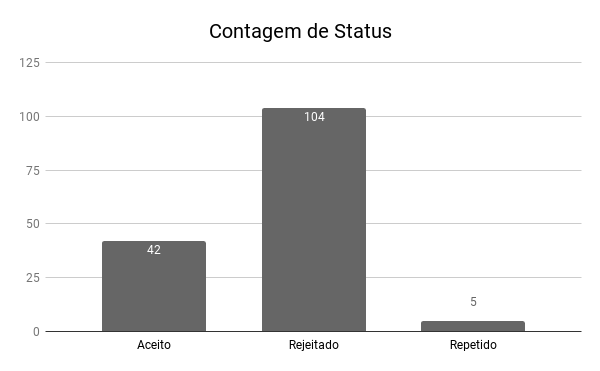
\includegraphics[width=0.8 \textwidth]{status.png}
% \caption{Contagem bases de dados \label{status}}
% \end{center}
% \end{figure}

\section{Resumo dos resultados encontrados}


\cite{mansini:2016} propôs uma técnica de programação matemática para solucionar o Problema de Roteamento de Enfermeiras, modelando o problema como uma variante do \textit{Multi-Vehicle Traveling Purchaser Problem} (MVTPP-PIC), elaborando uma solução a partir da abordagem \textit{Branch and Price}. Para realizar os testes computacionais, os autores geraram instâncias 10 novas instâncias para testar os algoritmos, adotando parcialmente o método de geração proposto para o MVTPP-PIC um artigo publicado por eles mesmos no ano anterior, encontrando uma solução ótima em três de  dez instâncias.

\cite{nguyen:2016} apresenta uma solução meta-heurística com base em Algoritmos Genéticos para solucionar o \ac{HHCP}. Em sua abordagem são utilizadas duas substituições: A primeira substitui as soluções anteriores aleatoriamente e a segunda substitui as piores soluções. Os testes computacionais foram realizados com instâncias baseadas em dados históricos reais de uma empresa de \textit{Home Care} que opera na Suíça.

% Foi proposta uma solução para o \ac{NSP}, baseado em Algoritmos Genéticos Cooperativos por \cite{ohki:2008}, tendo como solução um horário de enfermagem eficiente. Alguns anos depois \cite{ohki:2011} aplicou uma técnica de Penalização Ponderada em Algoritmos Genéticos Cooperativos para solucionar o \ac{NSP}, tendo como resultado o agendamento de horário realizado em um décimo do tempo, quando comparado com técnicas convencionais.

% Foi apresentado uma abordagem baseada em Memória Externa, junto com Algoritmos Genéticos Multi-Objetivos para resolver o \ac{NSP} por\cite{ahmet:2009}, tendo como resultado melhores soluções quando comparadas com os Algoritmos Genéticos Multi-Objetivos sem memória. 

\cite{tsai:2009} desenvolveram uma modelagem matemática em dois estágios para o \ac{PEE}, Na primeira etapa organiza-se o horário de trabalho e de folga das enfermeiras,  sendo utilizado uma abordagem baseada em Algoritmos Genéticos para resolver os horários. No segundo estágio, o cronograma das enfermeiras foi organizado e foi utilizado um  Algoritmo Genético com o objetivo de encontrar o horário ideal. O autor realizou um estudo de caso empírico, tendo como resultados que o Algoritmo Genético proposto pode ser uma ferramenta eficiente para resolver o \ac{NSP}.

 \cite{luna:2013} propuseram uma heurística para o Problema de Escalonamento de Equipe técnica baseada em Algoritmos Evolutivos, utilizando quatro instâncias reais, fornecidas por uma empresa privada. Os resultados mostram,  que o algoritmo proposto retornou resultados eficientes a partir da base de dados real utilizada e  que a paralelização proposta permite ao algoritmo abordar adequadamente instâncias com mais de 10000 instâncias. 

% Baseado na teoria Fuzzy, \cite{mutingi:2013}  elaborou uma heurística para o escalonamento de equipe de atendimento domiciliar, utilizando o método de Enxame de Particulas Fuzzy.
Em busca de encontrar a solução para o \ac{HHCSP}, \cite{trautsamwieser:2014} elaboraram uma heurística  \textit{Branch-Price-and-Cut} para o Problema. Em testes computacionais o autor testou sua abordagem com instâncias baseadas em mais de nove enfermeiras, 45 clientes e 203 visitas durante a semana.

Uma abordagem baseada em Programação por Restrições para o \ac{HHCP} foi elaborada por \cite{cattafi:2012}, Tendo como estudo de caso a realidade enfrentada pela cidade de Ferrara na Itália, onde o problema é resolvido manualmente. O autor formalizou o problema através da interação com a equipe de enfermagem do hospital da cidade, tendo como objetivo reduzir as disparidades nas jornadas de trabalho das enfermeiras.

\cite{bachouch:2010} descrevem um método para agendar tarefas e equilibrar a carga de trabalho dos profissionais do \ac{HHCSP} baseado na realidade dos hospitais da França. 

Foi desenvolvido uma solução heurística para solucionar o \textit{Crew Constrained Home Care Routing Problem with Time Windows} por \cite{tozlu:2016}, descrevendo o problema a partir de um modelo de programação linear misto e em seguida foi gerado aleatoriamente um conjunto de instâncias e resolvidos a partir do \textit{Variable Neighbourhood Search}. 

%Para encontrar uma boa solução para o \ac{NSP} \cite{kundu:2008} converteu o problema no Problema de Satisfação de Restrição e aplicou a técnica de Busca Local Gulosa incorporada com a Lista Tabu, testando também outras soluções baseadas no Restrição e aplicou o \textit{Simulated Anealing}, Algoritmo Genético, obtendo melhores resultados a partir da Busca Local Gulosa.
%Foi proposto por \cite{trabelsi:2012} um modelos de escalonamento baseado em Programação Interira Linear para fornecer soluções para o planejamento de curto prazo para o \ac{HHC}.

%Foi encontrada uma solução para o \textit{Therapist Routing and Scheduling Problem} a partir de um algoritmo sequencial adaptativo de Busca Gulosa Randomizada, o GRASP por \cite{bard:2012}, para testar sua solução foram realizados testes com dados reais fornecidos por uma empresa de reabilitação dos EUA, obtendo como resultado reduções de custo com uma média de cerca de 18,09\%.

Foi elaborado por \cite{Decerle:2016} uma heurística de duas fases para o \ac{HHCRSP} com o objetivo de reduzir custos relacionados a transporte e a horas trabalhadas pelos profissionais de saúde. Para solucionar o problema foram sugeridos duas abordagens: Um método de solução monofásica no qual um conjunto de dados é considerado como entrada para encontrar uma boa solução para o problema e uma meta-heurística em duas fases para distinguir o agendamento das enfermeiras. As abordagens são então aplicadas a várias instâncias de diferentes tamanhos, obtidas a partir de dois escritórios de \textit{Home Health Care} para compará-las.

Uma solução heurística proposta para o \ac{HHCP} por \cite{Bertels:2006} é baseada na combinação de Programação Linear Inteira, Programação por Restrição e meta-heurísticas. As instâncias utilizadas para gerar a solução foram obtidas a partir de 10 cenários sintéticos, contendo entre 20 e 50 profissionais e entre 111 e 326 trabalhos.

Foi elaborado por \cite{gambini:2012} uma solução heurística baseada em Programação Inteira para o \textit{International Nurse Rostering Competition}.

Foi elaborada por \cite{santos:2015} uma solução para o \ac{PEE} baseada em Programação por Restrição Ponderada, na qual dado uma série de restrições, visa minimizar o peso total de todas as restrições. Par a elaboração da solução os autores utilizaram uma variante do \ac{PEE} como um problema de vários estágios com 4 a 8 semanas, onde uma semana é considerada um estágio separado e individual. O objetivo da solução elaborada é atribuir um número fixo de enfermeiros a um conjunto de turnos. As restrições que devem ser satisfeitas pela solução elaborada pelos autoes são divididas em rígidas e flexíveis.
Após e execução dos testes os autores tiveram como resultado que, após cerca de 1000 passos, as restrições rígidas foram satisfeitas, as restrições flexíveis foram sendo resolvidas durante a fase de busca local.

% Foi elaborada uma heurística baseada em Busca Local para o \ac{NSP}, por \cite{inafune:2016}, os autores utilizaram em seus experimentos instancias reais, colhidas de um hospital.
% Foi elaborado por \cite{mutingi:2015} uma abordagem baseada em Algoritmo de Metamorfose Fuzzy para o \ac{NSP}, utilizando dados do mundo real e encontrados na literatura estudada.

\cite{constantino:2011} elaborou uma abordagem heurística para o \ac{NSP}, baseada em Satisfação de Preferência Balanceada. O algoritmo elaborado pelos autores possui duas fases: Na primeira fase é construída a solução inicial, resolvendo o problema sucessivo de atribuição por estrangulamento e na segunda fase são aplicados dois procedimentos de melhoria baseados em etapas de reatribuição. Os testes computacionais foram realizados com instâncias do \textit{Standard Benchmark Bataset} e a partir dos experimentos os autores concluíram que o método utilizado gerou resultados efetivos e eficientes para solucionar o problema.

% Foi formulada uma nova solução para o \ac{NSP} por \cite{baskaran:2014} utilizando o \textit{Branch and Bound} e o solucionador de simplex duplo, obtendo bons resultados a partir da aplicação de instâncias do mundo real.
% Uma abordagem colaborativa para resolver o \ac{NSP} foi elaborada por \cite{cares:2013} usando uma formulação de programação não-linear. Neste modelo, a função a ser otimizada é não-linear, esta função é focada em procurar uma solução que minimiza as diferenças entre os enfermeiros. Os autores utilizaram instâncias do mundo real para realizar os testes, obtendo resultados efetivos.

O algoritmo de Busca Harmônica  tem sido utilizado para solucionar problemas de otimização, este método funciona a partir da imitação do processo de improvisação musical.  Foi elaborada uma abordagem meta-heurística baseada em Busca Harmônica para o \ac{NSP}, por\cite{awadallah:2011}. Para realizar os testes computacionais foram utilizados dados do \textit{ International Nurse Rostering Competition 2010}, retornando bons resultados.

Foi desenvolvida um abordagem baseada em Programação Inteira Binária para gerar uma solução heurística para o \ac{NSP}, por \cite{Zen-El-Din:2012}. O autor realizou um estudo de caso  na unidade de terapia intensiva no Hospital do Cairo, sendo que os dados foram coletados de enfermeiros-chefe, supervisores, enfermeiros e assistentes.

Uma abordagem para resolver o \ac{NSP} em um hospital público na França foi desenvolvida por \cite{altamirano:2010} baseada em otimização por Enxame de Partículas, tendo resultados semelhantes em tempo computacional ao método de Programação Inteira e Programação por Restrição.

Foi elaborada uma heurística para o \ac{NSP} baseada em Vetorização de Matrizes por \cite{yindong:2008}, após experimentos computacionais foram obtidas boas soluções para 10 instâncias de dados reais de programação de enfermagem. 
Foi elaborado um modelo baseado em Lógica Fuzzy para solucionar o \ac{NSP} por \cite{topaloglu:2010}.
Um modelo de Programação Inteira Multi Objetivo para o \ac{NSP} foi proposto por \cite{cetin:2015}, em seguida os autores elaboram uma abordagem baseada em Lógica Fuzzy e aplicam a um estudo de cado em um hospital em Konya, na Turquia.

Foi elaborado por \cite{gutjahra:2007} uma heurística baseada em Colônia de Formiga para resolver o \ac{NSP} no \textit{Vienna Hospital Compound} na Áustria. Após realizar experimentos, foi observado que o algoritmo proposto alcança melhorias significativas em comparação a um algoritmo de abordagem gulosa.
Uma abordagem de otimização de Enxame de Particulas é proposto por \cite{wu:2015} para encontrar uma boa solução para o \ac{NRP}, tendo como estudo de caso um hospital de Taiwan. 

% É apresentado um modelo que integra  agendamento da enfermeira e do quarto cirúrgico e em seguida é mostrado por \cite{belien:2008} uma a abordagem da técnica de geração de coluna, um dos métodos exatos mais empregados para resolver problemas de programação de enfermeiros, pode fazer face facilmente a essa extensão de modelo.

Foi apresentado por \cite{lu:2012} um método baseado em \textit{Adaptive Neighborhood Search} para resolver o \ac{NSP} para do \textit{ First International Nurse Rostering Competition}.  Os resultados computacionais avaliados nos três conjuntos de 60 instâncias da competição mostram que o algoritmo utilizado melhora os resultados mais conhecidos por 12 instâncias ao combinar os melhores limites para outras 39 instâncias.

% Foi elaborado por \cite{burke:2010} um modelo de Programação Inteira e \textit{Variable Neighbourhood Search} para o Problema de Seleção de Enfermeiras, tendo como resultado boas soluções quando comparado com as soluções elaboradas com Algoritmos Genéticos e Busca em Vizinhança.

% Foi elaborado para a  Primeira Competição Internacional de Enfermagem (INRC2010),  uma abordagem em duas fases por \cite{valouxis:2012}, em sua solução na primeira fase, a carga de trabalho para cada enfermeiro e para cada dia da semana foi decidida, enquanto na segunda fase as deslocações diárias específicas foram atribuídas.

%\section{Análise descritiva dos resultados encontrados}

%Na seção anterior foi realizada uma revisão das soluções heurísticas encontradas a apartir da revisão sistemática de literatura, nessa parte serão descritas com mais detalhes algumas soluções heurísticas mais utilizadas pelos autores.

% \subsection{Técnicas de inteligência artificial}

% Vários autores utilizaram técnicas de inteligência artificial para elaborar heurísticas para o \ac{HHCSP} e o \ac{HHCRSP}, podendo citar as técnicas seguintes como as mais utilizadas.

%\subsection{Lógica Fuzzy}

% \
% \linebreak[4]

%A teoria de conjuntos difusos, do inglês \textit{fuzzy}, trabalha com modelos de conjunto cujo seus elementos possuem um determinado grau de pertinência a este conjunto, não aceitando valores booleanos, como acontece em conjuntos precisos, ou seja, que não são difusos \cite{mutingi:2013}.

%Para melhor entendimento sobre a teoria de conjuntos difusos, \citeonline{mutingi:2013} descreve a seguinte diferença entre os conjuntos:

%Seja um conjunto universo $X$ composto por elementos $x$, e o subconjunto $A$ do conjunto universo $X$, tal que $A \subseteq X$. 

%O elemento $x$ é um membro de um conjunto preciso se é definido pela função transformação $\mu_{A}$ a partir de $X$ em {0,1}, desde que:

% \begin{equation}
%  \mu_{A}(x) = 
%  \left \{
%  \begin{array}{cc}
%  1, & se \ x \ \in \ A  \\
%  0, & se \ x \ \notin \ A \\
%  \end{array}
%  \right.
%  \end{equation} 

%Em um conjunto difuso, o elemento $x \in A$  é definido por $\mu_{A}(x) \in [0,1]$, cujo cada elemento em X possui o valor dentro do intervalo [0,1] sendo que quanto mais próximo o valor de $\mu_{A}(x)$ está de $1$, maior é o grau de pertinência do elemento $x$ em A, e quanto mais próximo de $0$, menor o seu grau de pertinência.


%\subsection{Algoritmos Genéticos \hfill}
% \
% \linebreak[4]

%Algoritmos genéticos pertencem a uma subclasse de algoritmos evolutivos e possuem seu funcionamento baseado na teoria evolutiva da biologia proposta por Darwin. Nas ultimas décadas os algoritmos evolutivos tem sido bastante utilizados para resolver problemas de otimização.~\cite{malhotra:2011} 

%Os algoritmos genéticos contém um cromossomo, um gene, conjunto populacional, um \textit{fitness} e função \textit{fitness}, reprodução, mutação e seleção.

%O funcionamento dos algoritmos genéticos começam com um conjunto solução representado por um conjunto de cromossomos, chamado população, na qual cada cromossomo representa um individuo. As soluções são selecionadas de acordo com sua aptidão para gerar novas soluções, chamadas descendência, cada solução gerada para uma população é utilizada para uma nova população, possivelmente melhor do que a população anterior. 

%O processo utilizado para gerar uma população é repetido até que as condições pré definidas sejam satisfeitas, como pode ser visto no algoritmo~\ref{genetico}.

%\begin{algorithm}[ht]
% \Entrada{$P$} //população inicial \\
% \Saida{individuo que satisfaz a condição pré definida}
%   \Inicio{
%	Selecione uma subpopulacao $P'$
%     \While { $X$ não é satisfeito }{
%        escolha $S_{i}, S_{j} \in P'$ \\
%        $S_{k} \longleftarrow CRUZAMENTO(S_{i}, S_{j})$ \\
%      \eIf{$f(S_{i} \geq f(A_{j})$}{
%        	$S_{melhor} \longleftarrow S_{i}$\\
%        	}{$S_{melhor} \longleftarrow S_{j}$\\} 
%       \eIf{$f(S_{melhor}) \geq f(S_{k})$}{
%       	  $SUBSITUI(S_{melhor}, P)$\\
%        }{não substitui}  
%        $S_{k} \longleftarrow MUTACAO(S_{k})$ \\
%        }
%      \Retorna{$S_{k}$} \\
%   }
% \caption{Algoritmo genético \label{genetico}}
%\end{algorithm}

%O pseudocódigo acima ilustra o funcionamento do Algoritmo Genético, no qual a entrada é uma população P e a saída é um indivíduo $S$. Primeiramente é selecionada uma população inicial $P$ que irá gerar uma nova população. Até que o critério de parada seja satisfeitos, é gerada uma nova população $P'$, subconjunto da população $P$, da seguinte forma: São escolhidos aleatoriamente dois cromossomos $S_{i}$ e $S_{j}$ em cada subpopulação $P'$, estes cromossomos são recombinados a partir do cruzamento dos mesmos, levando a formação de um novo cromossomo $S_{k}$. O cromossomo $S$, representa o valor da função objetivo, dessa forma, quanto menor o valor, melhor será a adequação do indivíduo representado pelo cromossomo. Após a comparação do cromossomo filho com os cromossomos pais, é realizado o procedimento de mutação, gerando uma nova descendência.

%A cada iteração do algoritmo é testado se o indivíduo gerado satisfaz a condição $X$ pré definida, caso as condições sejam satisfeitas, o algoritmo para e retorna o indivíduo, caso contrário ele segue até que alcance alguma outra condição de parada $X$.

%\subsection{Memetic Algorithm}
% \
% \linebreak[4]

%\textit{Memétic Algorithm} são metaheurísticas baseadas em população, compostas por uma estrutura evolutiva e um conjunto de algoritmos de busca local. 
%Apesar de ser utilizado para resolver problemas de otimização, apesar de sua utilização o \textit{Memétic Algorithm} não é proposto como um algoritmo de otimização, mas como uma ampla classe de algoritmos inspirados pela difusão das ideias ideias e compostas por múltiplos operadores existentes~\cite{neri:2012}.  
 
%O \textit{Memétic Algorithm} visa a convergência de uma população para uma solução ótima, como segue:
%Primeiro é realizada a seleção aleatória das soluções candidatas iniciais, chamada de pais, que serão utilizadas para a criação de uma nova solução. Essa seleção é realizada levando em consideração o desempenho das soluções candidatas, quanto melhor o desempenho, maiores são as chances de seleção das soluções.
%A segunda etapa do algoritmo consiste em combinar os pais e criar uma nova solução candidata, mais próxima do resultado esperado.
%Após a geração da nova população, ocorre a fase de mutação, na qual é realizada uma melhoria no novo resultado gerado.   
%A ultima etapa decide se a nova população gerada deve se tornar membro da população e qual solução existente deve ser substituída.

%\subsection{Colônia de formiga}
% \
% \linebreak[4]

%O algoritmo de Colônia de Formigas, possui seu funcionamento baseado no comportamento das formigas na natureza, particularmente no processo realizado por estas ao procurar comida. Quando as formigas vão em busca de comida, elas partem aleatoriamente até encontrar a comida, ao encontrar a comida a formiga retorna para o seu ninho deixando uma trilha de ferormônios, que será seguida pelas outras formigas~\cite{blum:2005}.

%O algoritmo de Colônia de Formigas é descrito como um grafo G = (V,E), onde V consiste em dois nós nomeados $v_{s}$, representando o formigueiro e $v_{d}$, representando a comida; e $E$ representa duas ligações, $e_{1}$ e $e_{2}$ o caminho entre o formigueiro, representado por $v_{s}$ e a comida, representada por $v_{d}$. Sendo que $e_{1}$ representa o caminho mais curto e $e_{2}$ representa o caminho longo. 

%A representação da trilha de ferormônio é modelada da seguinte forma: É introduzido um ferormônio artificial $t_{i}$ para cada duas ligações $e_{i}$, sendo i=1,2; indicando a força da trilha deixada. Por fim, são introduzida formigas artificiais, representadas por $n_{a}$. Para criar o caminho de cada formiga do formigueiro até a comida, ou seja de $v_{s}$ para $v_{d}$, cada formiga que parte do ponto $v_{s}$ é escolhida com probabilidade: 

%\begin{equation}
%P{i} = {t_{i}\over\displaystyle {t_{1}+t_{2} } }, \ para\ i = 1,2
%\end{equation}

%entre os caminhos $e_{1}$ e $e_{2}$ para alcançar a comida $v_{d}$. Se $t_{1} > t_{2}$, a probabilidade do caminho 1 ser escolhido é maior.
%Para criar o caminho de volta para o formigueiro, ou seja, o caminho de $v_{d}$ para $v_{s}$ é utilizado o mesmo caminho criado de $v_{s}$ para $v_{d}$~\cite{blum:2005}.

%\subsection{Algoritmo Guloso}

%Algoritmos Gulosos sempre escolhem a melhor solução para o momento partindo do ótimo local em busca do ótimo global. Apesar deste algoritmo encontrar a solução ótima para vários problemas, nem sempre é possível alcançar a solução ótima a partir da execução deste algoritmo~\cite{Cormen:2009}. 

%Em um Algoritmo Guloso, a cada iteração, um novo elemento do conjunto solução é incorporado a construção da solução parcial até que a solução completa seja obtida. A seleção do próximo elemento que será incorporado é determinado a partir da função gulosa de avaliação. esta função gulosa representa o aumento incremental na função custo para a incorporação deste elemento na solução parcial em construção~\cite{resende:2014}. O critério para estabelecer qual elemento será selecionado é o do elemento menos custoso, como podemos ver no algoritmo~\ref{guloso}.

%\begin{algorithm}[ht]
% \Entrada{$C \neq \emptyset$} //conjunto de candidatos \\
% \Saida{melhor solução segundo o critério guloso}
%   \Inicio{
%   		$S \longleftarrow \emptyset $ //o conjunto solução $S$ está vazio inicialmente \\
%        $C \longleftarrow E $ //inicializa o conjunto $C$ com o conjunto inicial $E$ \\
%     \While {$C \neq \emptyset \wedge \neg solucao(S)$ }{
%        $ x \longleftarrow seleciona(C)$ //seleciona o proximo candidato \\
%        $C \longleftarrow C - x$ //remove x do conjunto de candidatos \\
%        \eIf{Viavel($S + x$)}{
%        	$S \longleftarrow S + x$  //adiciona o candidato ao conjunto solucao\\
%        }{$S \longleftarrow S$} //nao atualiza o conjunto solucao \\
     %}
%     \Retorna{S} //melhor solução segundo o critério guloso \\
%   }
% \caption{Algoritmo guloso  \label{guloso}}
%\end{algorithm}


%\subsection{Greedy Randomized Adaptative Search Procedure}
% \
% \linebreak[4]

%Para descrever o \ac{GRASP} será levado em consideração o problema de otimização combinatorial para minimizar a função $f(s)$ para cada solução $S \in X$, sendo definido a partir de um conjunto inicial finito $E = \{ e_{1}, e_{2}, ..., e_{n} \}$ para um conjunto viável de um conjunto soluções viáveis $X \subseteq 2^E$ e pela função objetiva $f:2^E\rightarrow$. 
%O conjunto de soluções viáveis para o problema é definido a partir do E, a função objetivo e das restrições. 
%O \ac{GRASP} é chamado de adaptativo porque os benefícios associados com cada elemento é atualizado a cada iteração da fase construtiva para refletir as mudanças trazidas pela seleção do elemento anterior.~\citeonline{resende:2014}.

%O \ac{GRASP} é definido por como uma heurística gulosa adaptativa de randomização iterativa constituída por duas fases: Uma fase construtiva e outra fase de busca local~\cite{feo:1995} e~\cite{resende:2014}. 
%Na fase de construção é elaborada uma solução, se esta solução não for viável, poderá ser descartada ou é aplicada uma heurística reparatória para alcançar a viabilidade. Uma vez que a solução viável é obtida, a vizinhança que possui esta solução é investigada até que seja encontrado o mínimo local através da etapa de busca local~\cite{resende:2014}.

% Para descrever o \ac{GRASP} \citeonline{resende:2014} leva em consideração o problema de otimização combinatorial para minimizar a função $f(s)$ para cada solução $S \in X$, sendo definido a partir de um conjunto solução finito $E = \{ e1, e2, ..., en \}$ para um conjunto viável de um conjunto soluções viáveis $X \subseteq 2^E$ e pela função objetiva $f:2^E\rightarrowR$. 
% O conjunto de soluções viáveis para o problema é definido a partir do E, a função objetivo e das restrições~\cite{feo:1995}.

%Para a elaboração da etapa construtiva, na qual solução viável é construída iterativamente, um elemento por vez e a cada iteração a escolha do próximo elemento que será adicionado é determinado pela ordem de todos os elementos candidatos em uma lista que respeita a função gulosa, são utilizados algoritmos randomizados.
%Os algoritmos randomizados são importantes para gerar o espaço de busca inicial em uma vizinhança, quebrar loops, habilitar trajetórias diferentes para seguir em uma mesma solução inicial ou simplificar diferentes partes em uma vizinhança extensa~\cite{resende:2014}. 

%Na fase de busca local, é utilizado um algoritmo de busca local que funciona de maneira iterativa, substituindo sucessivamente a solução corrente pela melhor solução encontrada na vizinhança, determinando quando a melhor solução não é encontrada na vizinhança.

%O algoritmo~\ref{grasp} ilustra o funcionamento do \ac{GRASP}, no qual recebe um conjunto de valores candidatos, o máximo de iterações e é utilizado um valor inicial pseudo-aleatório chamado semente e retorna a melhor solução encontrada.

%\begin{algorithm}[h]
% \Entrada{$C, m, s$} //conjunto de candidatos C, maximo de iteracoes m, e semente s \\
% \Saida{melhor solução}
%   \Inicio{
%		\For{$k \longleftarrow 1$ \KwTo $m$ }{
%        	$solucao \longleftarrow  %solucaoConstrutiva(C, s)$ \\
%            $solucao \longleftarrow  %buscaLocal(solucao, melhorSolucao)$\\
%        }
	
%     \Retorna{melhorSolucao} //melhor solução %segundo o critério guloso \\
%   }
% \caption{GRASP \label{grasp}}
%\end{algorithm}

%No contexto de atendimento do \ac{HHCSP} a heurística gulosa foi utilizada por alguns pesquisadores como~\cite{yuan:2015} e~\cite{bard:2012}, que utilizou o \ac{GRASP} para solucionar o \textit{Therapist Routing and Scheduling Problem}, problema semelhante ao \ac{HHCRSP}.

%\subsection{Adaptative Iterated Construction Search}
%não tem artigos falando sobre

%O \ac{AICS}, assim como o~\ac{GRASP}, é um algoritmo utilizado para resolver problemas de otimização, pertencente à sub-área de otimização cujo o conjunto de soluções viáveis é ou pode ser reduzido a um conjunto discreto. 
%Esse algoritmo utiliza a experiência adquirida em soluções passadas para gerar soluções melhores. 
%Uma forma de implementar esta ideia é associar pesos com possíveis decisões que serão tomadas durante o processo construtivo. Estes pesos são adaptados através de múltiplas iterações do processo de busca para refletir a experiência de iterações passadas~\cite{hoss:2005}.

%O funcionamento do \ac{AICS} é dividido em três fases: Construtiva, busca local e adaptação dos pesos. 
%Na fase construtiva, um processo de busca é utilizado para gerar uma solução candidata $s$, em seguida. 
%Na fase de busca local é realizada uma perturbação em $s$, produzindo a solução ótima local $s'$. 
%Por fim, os pesos são adaptados baseados nos componentes da solução utilizados em $s'$ e na qualidade da solução $s'$.
%O processo de busca construtiva utiliza o peso $w$ e alguma função heurística $h$ sobre os componentes da solução selecionados de componentes probabilisticamente selecionados para ampliar a solução parcial candidata atual. 
%Na fase de ajuste de pesos, é realizado um aumento dos pesos que correspondem aos componentes da solução em $s'$, podendo ser utilizados do histórico de busca~\cite{hoss:2005}.

%\subsection{Dynamic Local Search}

%A ideia geral do \ac{DLS} é buscar através do espaço de soluções viáveis e melhorar o retorno da função objetivo, realizando movimentos de subida para escapar de mínimos locais. Uma vantagem deste método é a rápia convergência em direção ao ótimo global da função objetivo sem utilizar derivadas de gradiente ou de ordem superior~\cite{amin:1997}.

%A ideia básica do algoritmo é explorar através do espaço local e global simultaneamente, permitindo a exploração detalhada de áreas de ótimos locais escapando destas.

%\subsection{Busca Tabu}
	
%A Busca Tabu é uma meta-heurística utilizada para guiar uma busca local na exploração do espaço solução além do ótimo local, sendo considerado um método cujo principal objetivo é minimizar a função objetivo $f(x)$~\cite{marti:2013}. A busca tabu é importante para resolver problemas de otimização utilizando uma estrutura de memória flexível~\cite{glover:1990}.
  
%Na busca tabu, é realizada uma busca na estrutura de vizinhança $N$, na qual a solução $x \in N(x)$ encontrada é trocada por uma solução melhor $x' \in N(x)$ atingida a partir de uma operação chamada movimento. 
%Este método permite apenas movimentos que melhorem o valor da função objetivo atual e a execução do algoritmo termina quando não são mais encontradas soluções melhores~\cite{marti:2013}. 
% O autor afirma que Uma falha existente no método decrescente é que o ótimo local, na maioria dos casos, não será o ótimo global, ou seja, geralmente não irá minimizar $f(x)$ em todas as soluções $x$ pertencentes a $X$.

%Na Busca Tabu são utilizados atributos flexíveis baseados em estruturas de memória que permitem a exploração do critério de avaliação e de informações de busca armazenadas; um mecanismo de controle associado, para empregar a estrutura de memória, com base na interação entre condições que restringem e liberam o processo de busca; e a incorporação das funções de memória de diferentes intervalos de tempo de curto a longo prazo, para implementar estratégias para intensificar e diversificar a busca.
%A memória de curto prazo, atribuída a Busca Tabu, constitui uma forma ativa de procurar o melhor movimento possível, sujeito a exigir escolhas disponíveis para satisfazer certas restrições. Estas restrições, que incorporam o limite tabu, são designadas para prevenir  movimentos reversos ou repetitivos e tem como objetivo principal das permitir que o método explore além do ótimo local enquanto mantém a qualidade dos movimentos em cada etapa. 
%Em várias aplicações a memória de curto prazo produz uma solução superior às encontradas com outros processos alternativos. Porém, a memória de longo prazo é importante para obter resultados para problemas mais difíceis. As memórias intermediárias e de longo prazo operam primeiramente como bases estratégicas para intensificar e diversificar a busca~\cite{glover:1990}.

%\subsection{Iterated Local Search}

%O ILS é um método utilizado para resolver problemas de otimização baseado em duas etapas que busca escapar de ótimos locais e alcançar a solução ótima global de forma mais eficiente possível.
%Para encontrar a solução candidata inicial, o ILS obtém a solução ótima local a partir da aplicação do procedimento de busca local. Cada iteração do algoritmo é composta por três estágios: Primeiro é aplicada uma pertubação à solução candidata atual $s$, gerando a solução candidata modificada $s'$; na segunda etapa é executada uma busca local auxiliar em $s'$, obtendo o ótimo local $s''$; na ultima etapa, um critério de aceitação é utilizado para selecionar a solução ótima dentre as soluções $s$ e $s''$~\cite{hoss:2005}. 

%\subsection{Branch and Bound}
  
%O funcionamento do \textit{Branch and Bound} é iniciado a partir de uma pesquisa em todo o espaço solução em busca da melhor solução para o problema.
%Cada iteração possui três componentes principais: O nó selecionado no processo, o calculo do limite (\textit{Bound}), e o ramo (\textit{Branch})~\cite{jean:1999}. 

%Iniciantemente o método \textit{Branch and Bound} considera um ponto qualquer no espaço de busca inexplorado onde será encontrado a melhor solução, este ponto inicial é chamado de conjunto raiz e a melhor solução é definida como infinito. Os subespaços inexplorados são representados por nós gerados dinamicamente e a cada iteração do \textit{Branch and Bound} é processado um nó.
%Em sequência é selecionado o próximo nó. Se a seleção do próximo nó é baseado no valor limite do subproblema, a primeira operação após escolher o nó é a criação de um novo ramo, subdividindo o subproblema em uma determinada quantidade de subespaços que serão investigados na próxima iteração. Para cada subespaço gerado é encontrado uma solução que é compara com a melhor solução atual, mantendo sempre a melhor solução.Caso seja determinado que determinado subespaço não possui a solução ótima, todo o subespaço é descartado~\cite{jean:1999}.

%\subsection{Constraint Programming}

%O problema de satisfação de restrição, consiste em um conjunto finito de variáveis, sendo que cada variável está associada a um valor e a um conjunto de restrições rígidas e flexíveis. A solução para o problema de satisfação por restrição é a satisfação de todas as restrições do domínio~\cite{maria:2008}.

% A diferença entre as restrições flexíveis e não flexíveis é o fato de que, se tratando das restrições flexíveis, o dano causado por sua violação é baixo ou nulo e as restrições não flexíveis devem ser satisfeitas obrigatoriamente \citeonline{blochiger:2003}.

%Existem três modelos computacionais baseados em restrições: Programação por restrições lógicas (\textit{Constraint Logic Programin}), programação restrita contínua( \textit{current Constraint Programming}), e programação restrita contínua pi-cálculo (\textit{concurrent Constraint Pi-calculus}).

%A programação por restrições lógicas é uma extensão da programação lógica, sendo ambas consideradas pertencentes ao paradigma declarativo, dessa forma o programador foca em o que computar ao invés de como computar. Esse método possui um conjunto finito de regras cujo corpo contem conjunções de literais, simbolo atômicos e restrições de domínio\cite{maria:2008}.

%A programação restrita contínua, conhecida como \textit{Current Constraint Programming}, possui a noção de armazenamento, representando o estado do sistema.
%Neste modelo o armazenamento é uma restrição que especifica uma informação parcial sobre possíveis valores de variáveis em qualquer estágio da computação. 
%A programação restrita contínua pi-cálculo,  \textit{Conncurrent Constraint Pi-calculus}, é um mecanismo síncrono e simétrico de interação entre quem envia e quem recebe os dados \cite{maria:2008}.

%A programação restrita contínua pi-cálculo (\textit{Conncurrent Constraint Pi-calculus}) é um mecanismo síncrono e simétrico de interação entre quem envia e quem recebe os dados.

%No contexto do \ac{HHCSP} vários autores como utilizaram o método \textit{Constraint Programming}, mais especificamente, programação lógica por restrições para encontrar boas soluções para o \ac{HHCSP} existindo algumas aplicações em casos particulares, como~\cite{bachouch:2010} e~\cite{cattafi:2012} que aplicaram a suas respectivas cidades.

%\subsection{Variable Neighborhood Search}

%O\ac{VNS} VSN explora uma vizinhança de forma a chegar cada vez mais distante da solução atual, trocando a solução atual por uma nova, se e somente se, a melhoria já foi feita, dessa forma, características de uma solução cuja varias variáveis já possuem seu valor ótimo, serão mantidas e usadas para obter uma boa vizinhança~\cite{hansen:2001}.

%Seja $N_{k} = (1, 2, ..., k_{max})$ um conjunto finito de estruturas de vizinhanças pré selecionadas, $N_{k}(x)$ um conjunto solução da vizinhança $k$ de $x$. A condição de parada é a máxima capacidade da CPU, o maior número de iterações, ou a maior quantidade de iterações entre duas melhorias. Geralmente, sucessivas vizinhanças $N_{k}$ estão aninhadas~\cite{hansen:2001}.

%O funcionamento do VNS é como segue: 
%Na fase de inicialização é selecionado um conjunto de estruturas de vizinhanças $N_{k} = (1, 2, ..., k_{max})$ que será utilizado na busca; escolhido a solução inicial $x$ e a condição de parada.
%Em seguida repete-se até a condição de parada os seguintes passos:
%1 - O conjunto $k$ é inicializado com $1$;
%2 - Até que $k = k_{max}$, repete-se os seguintes passos:
%    a. Gera um ponto $x'$ aleatoriamente em qualquer das vizinhanças de $x$
%    b. Aplica-se algum algoritmo de busca local com $x'$ como solução inicial
%    c. Se o ótimo local for melhor que a solução atual, então move $x <- x''$, continua a busca em $N_{1}(k<-1)$, caso contrário $k <- k+1$;

%\subsection{Variable Depth Search}

%O VDS é um método de melhoria iterativa no qual as etapas de busca local são variáveis sequências de passos de busca simples em uma pequena vizinhança. As restrições nas sequências viáveis em passos simples auxiliam a manter a complexidade do algoritmos baixa~\cite{hoss:2005}.

%O funcionamento do VDS inicia-se a partir da criação de uma lista inicial, escolhida a partir da utilização do método \textit{Randomized Greedy Assignemnt Method}. A cada troca que deve ser realizada, é escolhido o item que possui o menor ganho em penalidade, Para fornecer diferentes soluções iniciais e permitir que a busca também seja usada com reinícios aleatórios, o conjunto de turnos que serão atribuídos é embaralhado. Uma vez que a lista inicial é criada, é possível prosseguir com o \ac{VDS}~\cite{burke:2013}.

% \section{Considerações}

% A partir da análise das heurísticas utilizadas pelos autores pesquisados para resolver o problema de roteamento e escalonamento de profissionais da área da saúde, pode-se concluir que foram utilizados diversos métodos heurísticos para encontrar boas soluções para o problema, como Busca local, técnicas de Inteligência Artificial, Análise de Vizinhança, Programação por Restrição e  Algoritmos Gulosos.